\documentclass{article} % Tipo de documento

\usepackage[utf8]{inputenc} % Permite el uso de caracteres del Español

\usepackage[T1]{fontenc}

\usepackage{graphicx}

% Carátula del Artículo  

\title{Reporte de Actividad 1}

\author{Brenda Leyva Amaya}

\date{30 de Enero, 2018}
 

\begin{document}

\maketitle % Crea el título


\section{Introducción}

	El presente documento contiene valiosa información acerca de la atmósfera de la tierra, el cual se ha creado con el fin de poner en práctica varias habilidades, tanto como el uso del lenguaje \LaTeX, así como la lectura en lengua extranjera y la capacidad de redacción de textos de índole científica.
\vspace{0.5 cm}

    Esta actividad representa el primer acercamiento al curso de física computacional de la licenciatura en Física de la Universidad de Sonora. 

\section{La atmósfera terrestre}

 \begin{center}
 	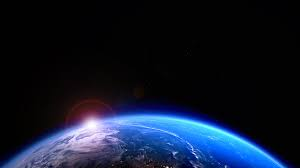
\includegraphics[width=8cm]{index.jpeg}
    
    Tierra vista desde el espacio.
 \end{center}

	La atmósfera de la tierra es una capa de gases, comunmente conocidos como aire, que rodea al planeta tierra y se mantiene en su lugar debido a la fuerza de gravedad del planeta. La atmósfera de la tierra protege la vida en ella al crear cierta presión que permite que el agua exista en estado líquido en la superficie, absorbiendo la radiación solar ultravioleta, también calienta la superficie al retener calor por medio del efecto invernadero. A su vez la atmósfera reduce las temperaturas extremas entre día y noche. 
\vspace{0.5 cm}

	El estudio de la atmósfera de la tierra y sus procesos se llama ciencia atmosférica o aerología. Los pioneros en este campo incluyen León Teisserenc de Bort y Richard Assmann.

\subsection{Composición}

	Los tres principales constituyentes del aire, y por lo tanto de la atmósfera son el nitrógeno, el oxígeno y el argon. El valor de agua constituye un 0.25\% de la masa de la atmósfera. La concentración de vapor de agua, que es un gas de efecto invernadero, varía significativamente de aproximadamente 10 ppm por volumen en las partes más frías de la atmósfera hasta tanto como el 5\% por volumen en las masas de aire caliente y húmedo. Concentraciones de los otros gases atmósfericos se denominan tipicamente en términos de aire seco, o aire sin vapor de agua. 
\vspace{0.5 cm}

	Es común referirse al resto de los gases como gases remanentes, entre los cuales se encuentran los grases de efecto invernadero, principalmente dioxido de carbono, metano, óxido nitroso y ozono. El aire filtrado incluye restos de muchos compuestos químicos. Algunas substancias de orígen natural pueden estar presentes en cantidades variables incluyendo polvo de composición mineral y orgánica, polen, esporas, brisa del mar y ceniza volcánica. Sin embargo también se pueden encontrar contaminantes de orígen industrial como gases y aerosoles.

\begin{center}

 	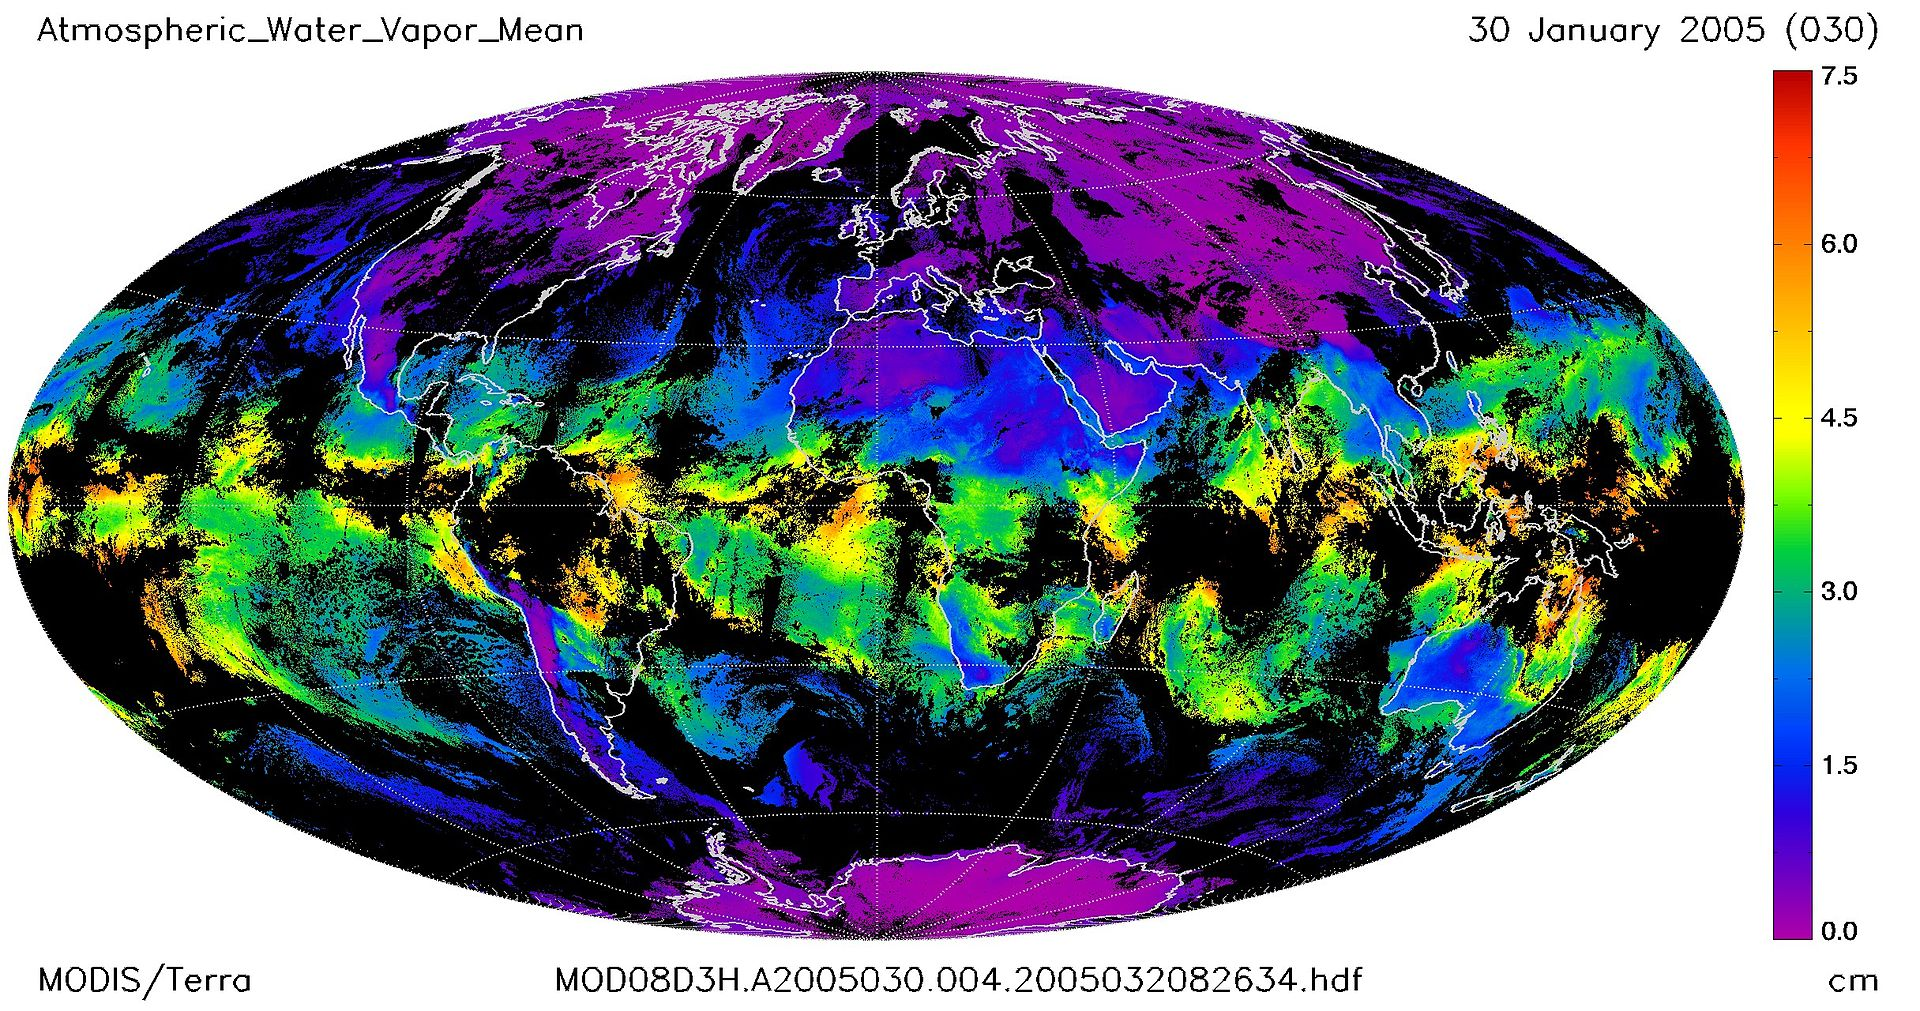
\includegraphics[width=10cm]{watervapor.jpg}
    
    Promedio de vapor de agua.
    
 \end{center}


\subsection{Estructura de la atmósfera}

En general, la presión y densidad del aire disminuye con la altitud en la atmósfera. Sin embargo, la temperatura tiene un perfil más complicado en referencia con la altitud y puede permanecer relativamente constante o incluso aumentar con la altitud en algunas regiones. Debido a que el patrón general de la temperatura con respecto a la altitud es constante y medible, el comportamiento de la temperatura proporciona una referencia útil para distinguir las distintas capas de la atmósfera. 
\vspace{0.5 cm}

	De esta manera, la atmósfera se puede dividir en cinco principales capas. Excluyendo la exósfera, la atmósfera tiene cuatro principales capas, que son la tropósfera, la estratósfera, mesósfera y termósfera. 
\vspace{0.5 cm}

	De la de mayor altitud a la mas baja, las cinco capas son:
\vspace{0.5 cm}

    Exósfera: 700 to 10,000 km (440 to 6,200 miles)
\vspace{0.5 cm}

    Termósfera: 80 to 700 km (50 to 440 miles)
\vspace{0.5 cm}

    Mesósfera: 50 to 80 km (31 to 50 miles)
\vspace{0.5 cm}

    Estratósfera: 12 to 50 km (7 to 31 miles)
\vspace{0.5 cm}

    Tropósfera: 0 to 12 km (0 to 7 miles)
\vspace{0.5 cm}

	Dentro de las cinco principales capas que están determinadas principalmente por la temperatura, se pueden distinguir varias capas secundarias en base a otras propiedades. La capa de ozono se encuentra contenida en la estratósfera. En esta capa, las concentraciones de ozono son de entre 2 y 8 partes por millón, lo cual es mucho más alto que en la atmósfera baja pero aún así pequeño en comparación con los principales componentes de la atmósfera. 
\vspace{0.5 cm}

    La ionósfera es una región de la atmósfera que está ionizada por la radiación solar. Esta capa es la responsable de que existan auroras boreales. La ionósfera se forma en el extremo interno de la magnetósfera. Tiene importancia práctica pues tiene influencia, por ejemplo en la propagación de ondas de radio en la tierra. La homósfera y la heterósfera están definidas según lo bien que esten mezclados los gases atmosféricos. La temperatura promedio de la atmósfera es 14 grados centígrados.


\subsection{Propiedades físicas}

\vspace{0.5 cm}

\begin{center}

 	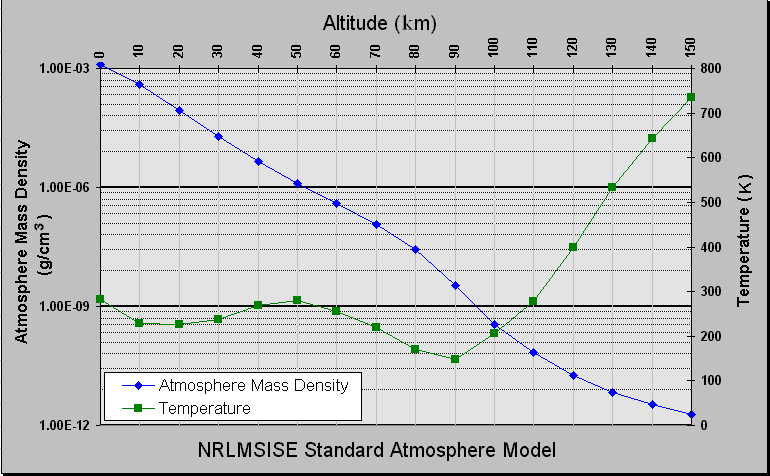
\includegraphics[width=10cm]{Atmosphere_model.png}    
    
\end{center}

\textbf{Presión y grosor}
\vspace{0.5 cm}

La presión promedio de la atmósfera a nivel del mar se define por el Estándar Internacional como 101,325 pascales. Algunas veces se refiere a esto como la unidad estándar en atmósferas (atm). La masa atmosférica total es 5.1480x1018 kg, aproximadamente 2.5\% menos de lo que se podría inferir del la presión promedio a nivel del mar y el área de la tierra de 5,1007.2 mega-hectáreas. La presión atmosférica es el peso total del aire sobre una unidad de área en un punto donde la presión es conocida. Así la presión del aire varía con la ubicación y el clima.  
\vspace{0.5 cm}

	En resumen, la masa de la atmósfera de la tierra está distribuida aproximadamente como sigue:
\vspace{0.5 cm}

    50\% está debajo de 5.6 km (18,000 ft).
\vspace{0.5 cm}
    
    90\% está debajo de 16 km (52,000 ft).
\vspace{0.5 cm}
    
    99.99997\% está debajo de 100 km (330,000 ft)
\vspace{0.5 cm}
    
    Por convención internacional está última marca el comienzo del espacio donde los viajantes humanos son considerados astronautas. 
\vspace{0.5 cm}
   
	A manera de comparación, la cima del Monte Everest está a 8,848 m (29,029 ft); aerolineas comerciales típicamente viajan entre 10 km (33,000 ft) y 13 km (43,000 ft) donde el aire más ligero mejora el desempeño del combustible.
\vspace{0.5 cm}

\textbf{Temperatura y velocidad del sonido. }
\vspace{0.5 cm}

	En la atmósfera la temperatura disminuye con la altitud comenzando a nivel del mar, pero variaciones en esta tendencia ocurren por encima de los 11 km de altitud, donde la temperatura se estabiliza a través de una amplia distancia vertical en el resto de la tropósfera. En la estratósfera, comenzando en aproximadamente 20 km, la temperatura aumenta con el peso, esto debido a un calentamiento en la capa de ozono causado por un almacenamiento significativo de radiación ultravioleta del sol en esta región. Además otra región de aumento de temperatura ocurre a grandes altitudes en la termósfera por encima de los 90 km.
\vspace{0.5 cm}

	Debido a que en un gas ideal de composición constante la velocidad del sonido depende solo de la temperatura y no en la presión o densidad del gas, la velocidad del sonido en la atmósfera con la altitud toma la forma de un complejo perfil de temperatura y no iguala cambios en densidad o presión relacionados con la altitud. 
\vspace{0.5 cm}

\textbf{Masa y densidad.}
\vspace{0.5 cm}

La densidad del aire al nivel del mar es aproximadamente 1.2 kg/m3. La densidad no se mide directamente, si no que es calculada desde mediciones de temperatura, presión y humedad, utilizando la ecuación de estado para el aire. La densidad atmosférica disminuye a medida que la altitud aumenta. Esta variación se puede modelar con la formula barométrica. Algunos modelos más sofisticados se utilizan para predecir la órbita de los satélites. 
\vspace{0.5 cm}

La masa promedio de la atmósfera es de aproximadamente 1/1,200,000 la masa de la tierra. De acuerdo con el Centro Nacional Americano para la Investigación atmosférica, "La masa promedio total de la atmósfera es $5.1480x10^{18}$ kg.

\subsection{Propiedades ópticas}

\vspace{0.5 cm}

\begin{center}

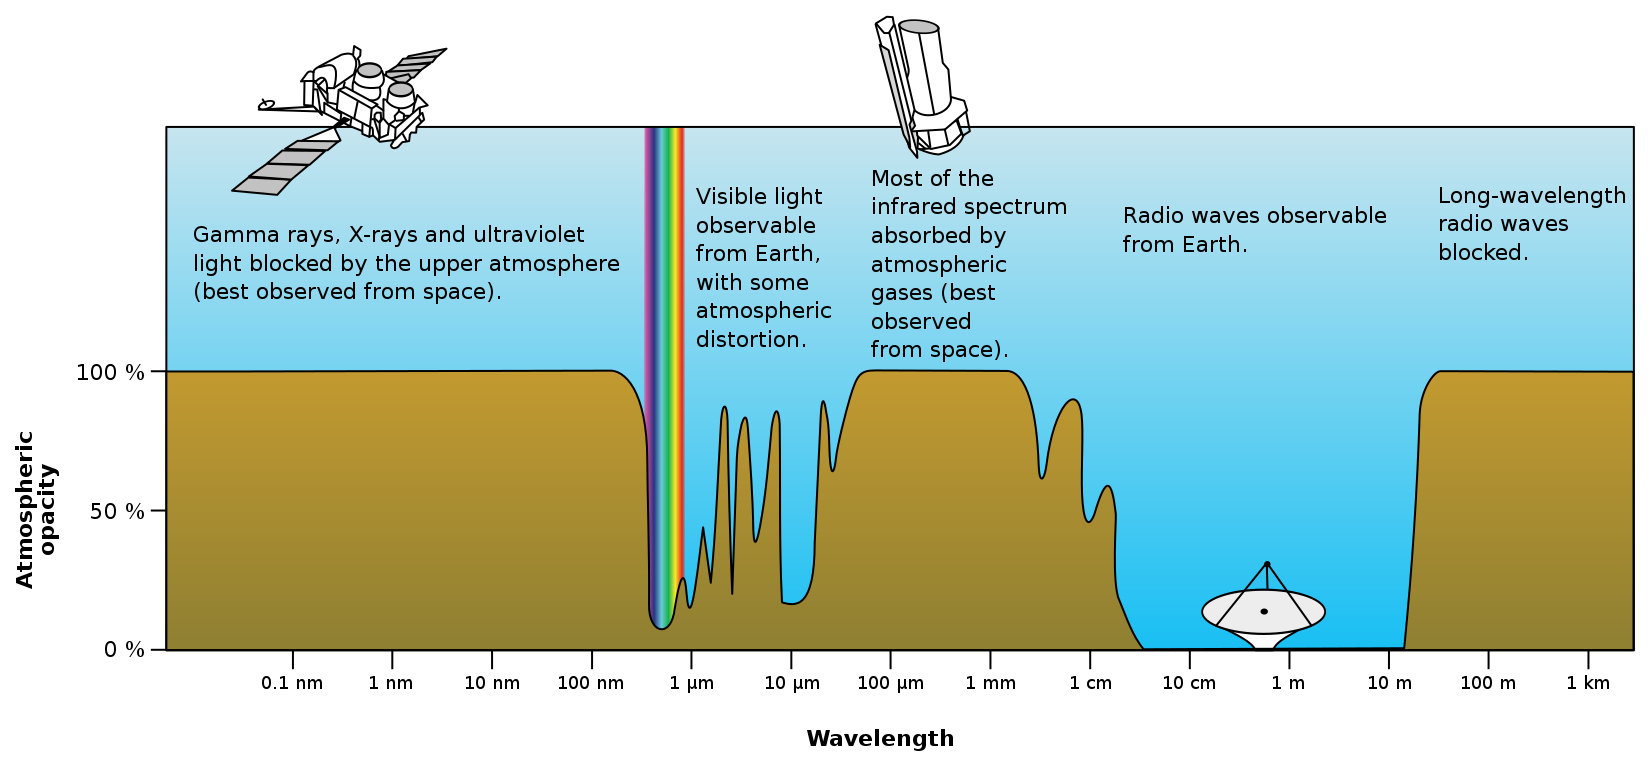
\includegraphics[width=12cm]{Atmospheric_electromagnetic_opacity_svg.png}    
    
\end{center}

La radiación solar es la energía que la Tierra recibe del sol. La Tierra a su vez emite radiación hacia el espacio, pero a longitudes de onda mayores que no podemos ver. Parte de la radiación que entra y sale se absorbe o es reflejada por la atmósfera. Cuando la luz pasa a través de la atmósfera de la Tierra, los fotones interactúan con ella al ser esparcida. Si la luz no interactúa con la atmósfera, se le llama radiación directa y es lo que vemos si observamos directamente el sol. La radiación indirecta es luz que se ha esparcido en la atmósfera. Por ejemplo en un día nublado cuando no se puede ver la sombra, se dice que no hay radiación directa alcanzandote. 
\vspace{0.5 cm}

Diferentes moléculas absorben diferentes longitudes de onda de la radiación. Por ejemplo O2 y O3 absorben casi todas las longitudes de onda menores a 300 nanometros. El agua absorbe una gran cantidad de longitudes de onda por encima de los 700 nanometros. Cuando una molécula absorbe un fotón, este aumenta la energía de dicha molécula, este efecto calienta la atmósfera pero esta a su vez se enfría al también emitir radiación. 
\vspace{0.5 cm}

La emisión es lo opuesto a la absorción, esta se dá cuando un objeto emite radiación. Los objetos tienden a emitir cantidad y longitudes de onda de radiación dependiendo de sus curvas de radiación de cuerpo negro, por lo tanto objetos más calientes tienden a emitir más radiación con longitudes de onda más cortas. Los objetos más fríos emiten menos radiación con longitudes de onda mayores. Debido a su temperatura la atmósfera emite radiación infraroja. El efecto invernadero está directamente relacionado a esta absorción y emisión. Algunos gases en la atmósfera absorben y emiten radiación infraroja, pero no interactúan con la luz del sol en el espectro visible, ejemplos de estos son las moléculas de CO2 y H2O.
\vspace{0.5 cm}

El índice de refracción del aire es cercano a 1. Variaciones sistemáticas en el índice de refracción pueden llevar a la distorción de los rayos de luz sobre caminos ópticos largos. Un ejemplo de esto es que, bajo ciertas circunstancias, los observadores a bordo de barcos pueden ver otras naves justo sobre la linea del horizonte, ya que la luz se refracta en la misma dirección que la curvatura de la superficie de la Tierra. 

\subsection{Circulación}

La circulación atmosférica es el movimiento a gran escala del aire a tráves de la tropósfera y la manera en que por medio de la circulación del aire oceánico el calor se distribuye alrededor de la Tierra. Esta mega estructura varía de año a año, pero su constitución básica se mantiene relativamente constante ya que depende de la rotación de la Tierra y la diferencia en radiación solar entre el ecuador y los polos. 
\vspace{0.5 cm}

\begin{center}

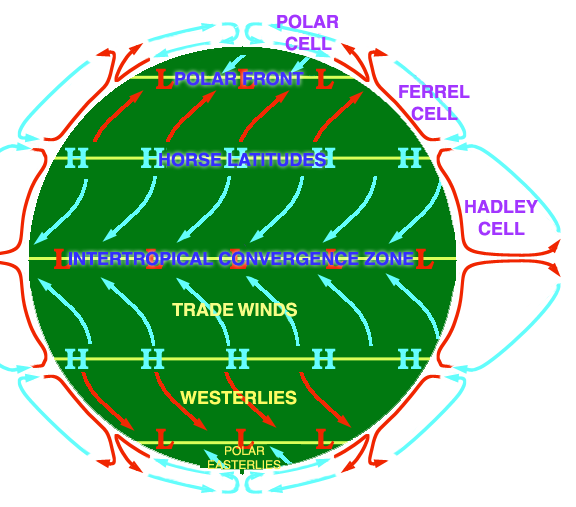
\includegraphics[width=8cm]{AtmosphCirc2.png}    
    
\end{center}

\vspace{5cm}

\section*{Bibliografía y fuentes}

Atmosphere of Earth. (2018, January 17). Retrieved January 24, 2018, from $https://en.wikipedia.org/wiki/Atmosphere_of_Earth$

\vspace{0.5cm}


\section*{Apéndice 1}

\hspace{0.45 cm} ¿Qué fue lo que más te llamó la atención de esta actividad?

\vspace{0.5 cm}
Me pareción muy interesante la información que se revisó pues es un tema al cual no había tenido exposición en algunos años y es información no solo útil pero también atractiva y con cierto carácter de entretenimiento. También fué bueno poner en práctica la traducción rápida y efectiva de textos en inglés a español. 
\vspace{0.5 cm}

¿Qué fue lo que se te hizo menos interesante?

\vspace{0.5 cm}
De todo lo que realizamos, la creación de este apéndice es la que me pareción menos interesante, pero no por ello se le ha de restar importancia a la reflexión.
\vspace{0.5 cm}

¿Qué cambios harías para mejorar esta actividad? 

\vspace{0.5 cm}
Para lograr una mejora significativa de los resultados que se obtuvieron sería necesario familiarizarme mucho más con las diferentes posiblidades de \LaTeX así se podría realizar un documento de mayor calidad y con mejores aspectos visuales. 
\vspace{0.5 cm}

¿Cuál es tu primera impresión de uso de \LaTeX?

\vspace{0.5 cm}
Es una manera muy efectiva de realizar trabajos que tengan una mejor presentación y cuya modificación y el añadir diferentes funciones es mucho más sencilla y efectiva que con un software de edición de texto regular.  
\vspace{0.5 cm}

¿El tiempo sugerido para esta actividad fue suficiente? 

\vspace{0.5 cm}
El tiempo me pareción más que suficiente y adecuado.
\vspace{0.5 cm}

¿Encontraste algún documento o recurso en línea útil que quisieras compartir con los demás?  

\vspace{0.5 cm}
No se llevó a cabo investigación adicional acerca del tema.
\vspace{0.5 cm}

 
 
 
\end{document}